\\ \\
Lezione 08/04, ultima modifica 20/05, Michele Nardin
\\ \\
\noindent \textbf{Esempio di test bilaterale}
Sia $(X_1,...,X_n)$ un campione casuale da una distribuzione avente media $\mu$ e varianza $\sigma^2$ finite. 
Considerato il fatto che non abbiamo informazioni sulla distribuzione delle variabili casuali, 
ci appoggeremo su di un test \textit{approssimato}.
Supponiamo di voler verificare la seguente ipotesi relativa alla media della distribuzione:

$$\bigg \{
\begin{array}{rl}
H_0: & \mu = \mu_0 \\
H_1: & \mu \neq \mu_0 \\
\end{array}
$$
\\ \\
Seguendo la falsariga di quanto visto sopra, procediamo come segue:

\begin{enumerate}
\item [(a)] Prendiamo $\overline{X}=\displaystyle \frac{\sum X_i}{n}$, che è stimatore della media del campione. Non conoscendo la distribuzione esatta delle variabili, consideriamo la distribuzione approssimata: sotto $H_0$ abbiamo che $\overline{X} \stackrel{a}{\sim} N(\mu_0,\sigma^2 / n) $ (questo, come già detto varie volte, per il TLC).

\item [(b)] Scegliamo una regola di decisione: usando anche la distribuzione asintotica di $\overline{X}$ sotto $H_0$, individuiamo la \textit{regione di rifiuto del test}. 
Dobbiamo trovare quindi due valori $h,k \in \mathbb{R}$ 
tali per cui \textit{rifiuto} $H_0$ se $\overline{X_n} \leq h$ o $\overline{X_n} \geq k$.

\item [(c)] Scelto il livello di confidenza $\alpha$, si ha che $h,k$ vanno scelti in modo tale per cui 
$$\alpha = P(\overline{X} \leq h \vee \overline{X} \geq k \mid \mu=\mu_0)$$
Grazie alla normalità della distribuzione asintotica, possiamo supporre che la distribuzione di $\overline{X_n}$ sia simmetrica, per lo meno da un certo $n$ in poi (ricordiamo che, per campioni con numerosità superiori a 30, l'approssimazione è già buona).

Questo ci permette di scrivere
$$\frac{\alpha}{2} = P(\overline{X} \leq h \mid \mu=\mu_0) = P(\overline{X} \geq k \mid \mu=\mu_0)$$

Dato che $$\frac{\overline{X} - \mu_0}{S_n / \sqrt{n}} \stackrel{D}{\to} N(0,1)$$
denotato con $z_{\alpha/2}$ il quantile di ordine $\alpha / 2$ della normale standard, la regione critica (di rifiuto) sarà
$$C=\left\{ \underline{x}=(x_1,...,x_n) \in X : \left| \frac{\overline{X} - \mu_0}{S_n / \sqrt{n}} \right| \geq z_{\alpha/2} \right\}$$
da cui $$k =  \frac{S_n}{\sqrt{n}}z_{\alpha/2} + \mu_0 (= -h )$$
\end{enumerate}

Consideriamo inoltre la funzione di potenza associata, sempre sfruttando l'approssimazione normale ed il fatto che, per n grande, $S_n \approx \sigma$:

\begin{align*}
\gamma(\mu) &=P(\overline{X} \leq \mu_0 - \frac{S_n}{\sqrt{n}}z_{\alpha/2} \mid \mu \neq \mu_0 ) 
+ P(\overline{X} \geq \mu_0 + \frac{S_n}{\sqrt{n}}z_{\alpha/2} \mid \mu \neq \mu_0 )
\\ & \approx \Phi\left( \frac{\sqrt{n}(\mu_0 - \mu)}{\sigma} - z_{\alpha / 2} \right)
 + \left[ 1 - \Phi\left( \frac{\sqrt{n}(\mu_0 - \mu)}{\sigma} - z_{\alpha / 2} \right) \right]
\end{align*}
Di seguito possiamo osservare il grafico della funzione:\\
\begin{center}
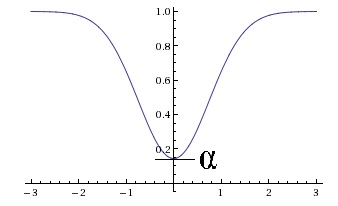
\includegraphics {immagini/potenza_bilaterale.jpg}
\end{center}

\textbf{Osservazione:} i test costruiti usando t di Student sono più conservativi rispetto a quelli costruiti con approssimazione Normale, nel senso che è più facile che un test venga accettato usando la prima rispetto alla seconda. Questo è dato dal fatto che la distribuzione t di student ha le code più pesanti rispetto alla normale! (in particolare fissato un 
$\alpha \in (0,1)$,
 i quantili della normale standard $z_{\alpha/2}$ sono più piccoli dei quantili della t di Student con $n-1$ gradi di libertà $t_{\alpha/2; n-1}$, cioè 
$|z_{\alpha/2}| < |t_{\alpha/2; n-1}|$)
\\ \\
